% !TEX root = ../../../Masterthesis.tex

\chapter{Star Trek VIII: First Contact}\label{ch:st 8}

\section{Main Title}
%-----------------------------------------------------------------------------
% Introduction, A and B
%-----------------------------------------------------------------------------
\begin{figure}[h!]
\center
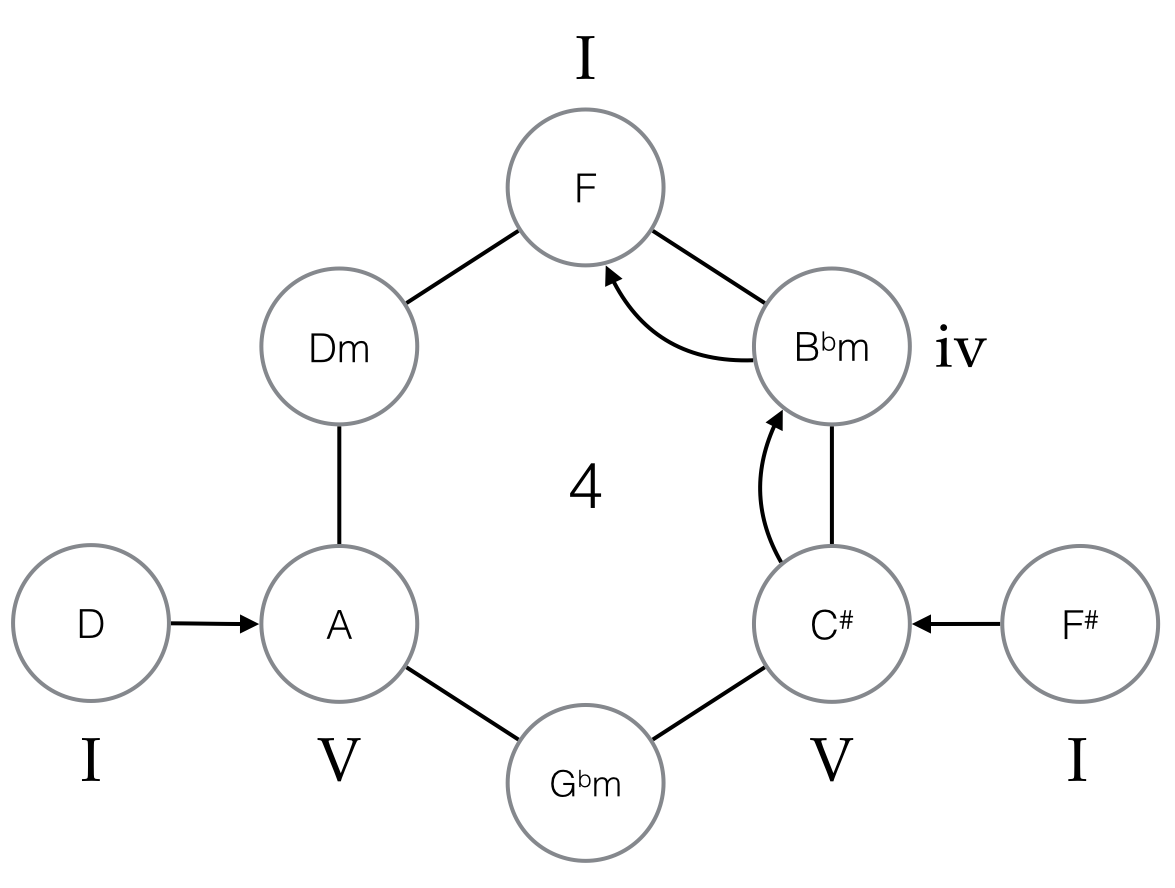
\includegraphics[width=0.7\linewidth]{ST8_introduction}
	\caption{ST 8: Introduction}
	\label{ST8_introduction}
	\setfloatalignment{b}
\end{figure}

\noindent\newthought{In direct opposition} to the tone of the movie, the main title of Star Trek: First Contact provides an emotionally charged and inspiring tone. The introduction, figure \ref{ST8_introduction}, treats us with the Star Trek theme twice, first in D-A and then in \fiss-\ciss, quickly moving down through \bflatm to F, which one might describe as a plagal cadence with minor subdominant. The tonal energy in A and B is very much centered around the well established \(I-IV-V\) and \(vi-IV-ii-V-I\) cycles. 
%-----------------------------------------------------------------------------
% C
%-----------------------------------------------------------------------------
From m. 28 Goldsmith executes a modulation to the dominant C and repeats \(ii-V\) twice before moving to Cm. He then executes a Aeolian Cadence, figure \ref{ST8_aeolian_cadence}, modulating to F major and ending on the dominant C in m.35. The main theme of the cue repeats once more ending with a lydian, ``fantastical'' sounding progression. 
\begin{marginfigure}
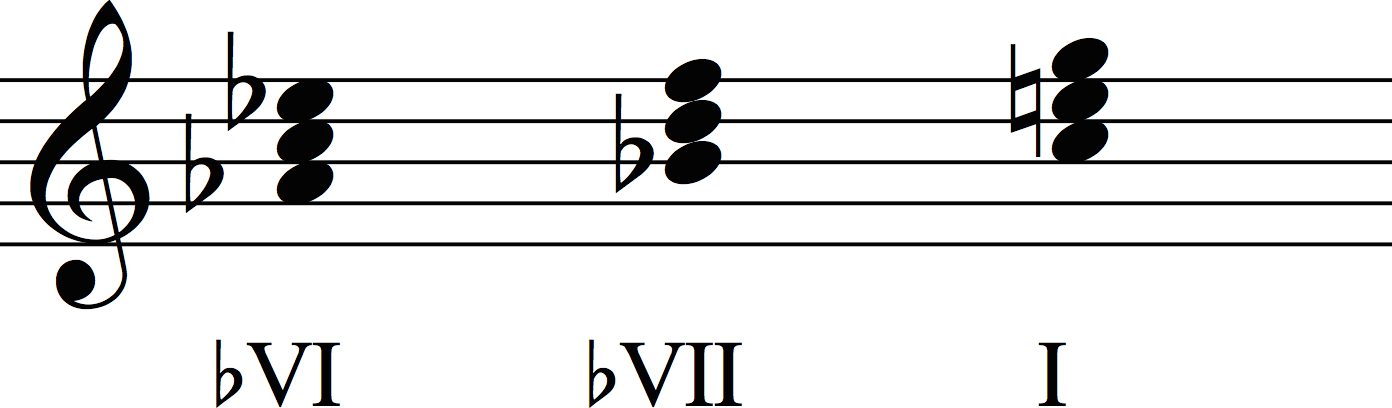
\includegraphics[width=\linewidth]{ST8_aeolian_cadence}
	\caption{Aeolian Cadence}
	\label{ST8_aeolian_cadence}
	%\setfloatalignment{b}
\end{marginfigure}

%-----------------------------------------------------------------------------
% PDF
%-----------------------------------------------------------------------------
\clearpage
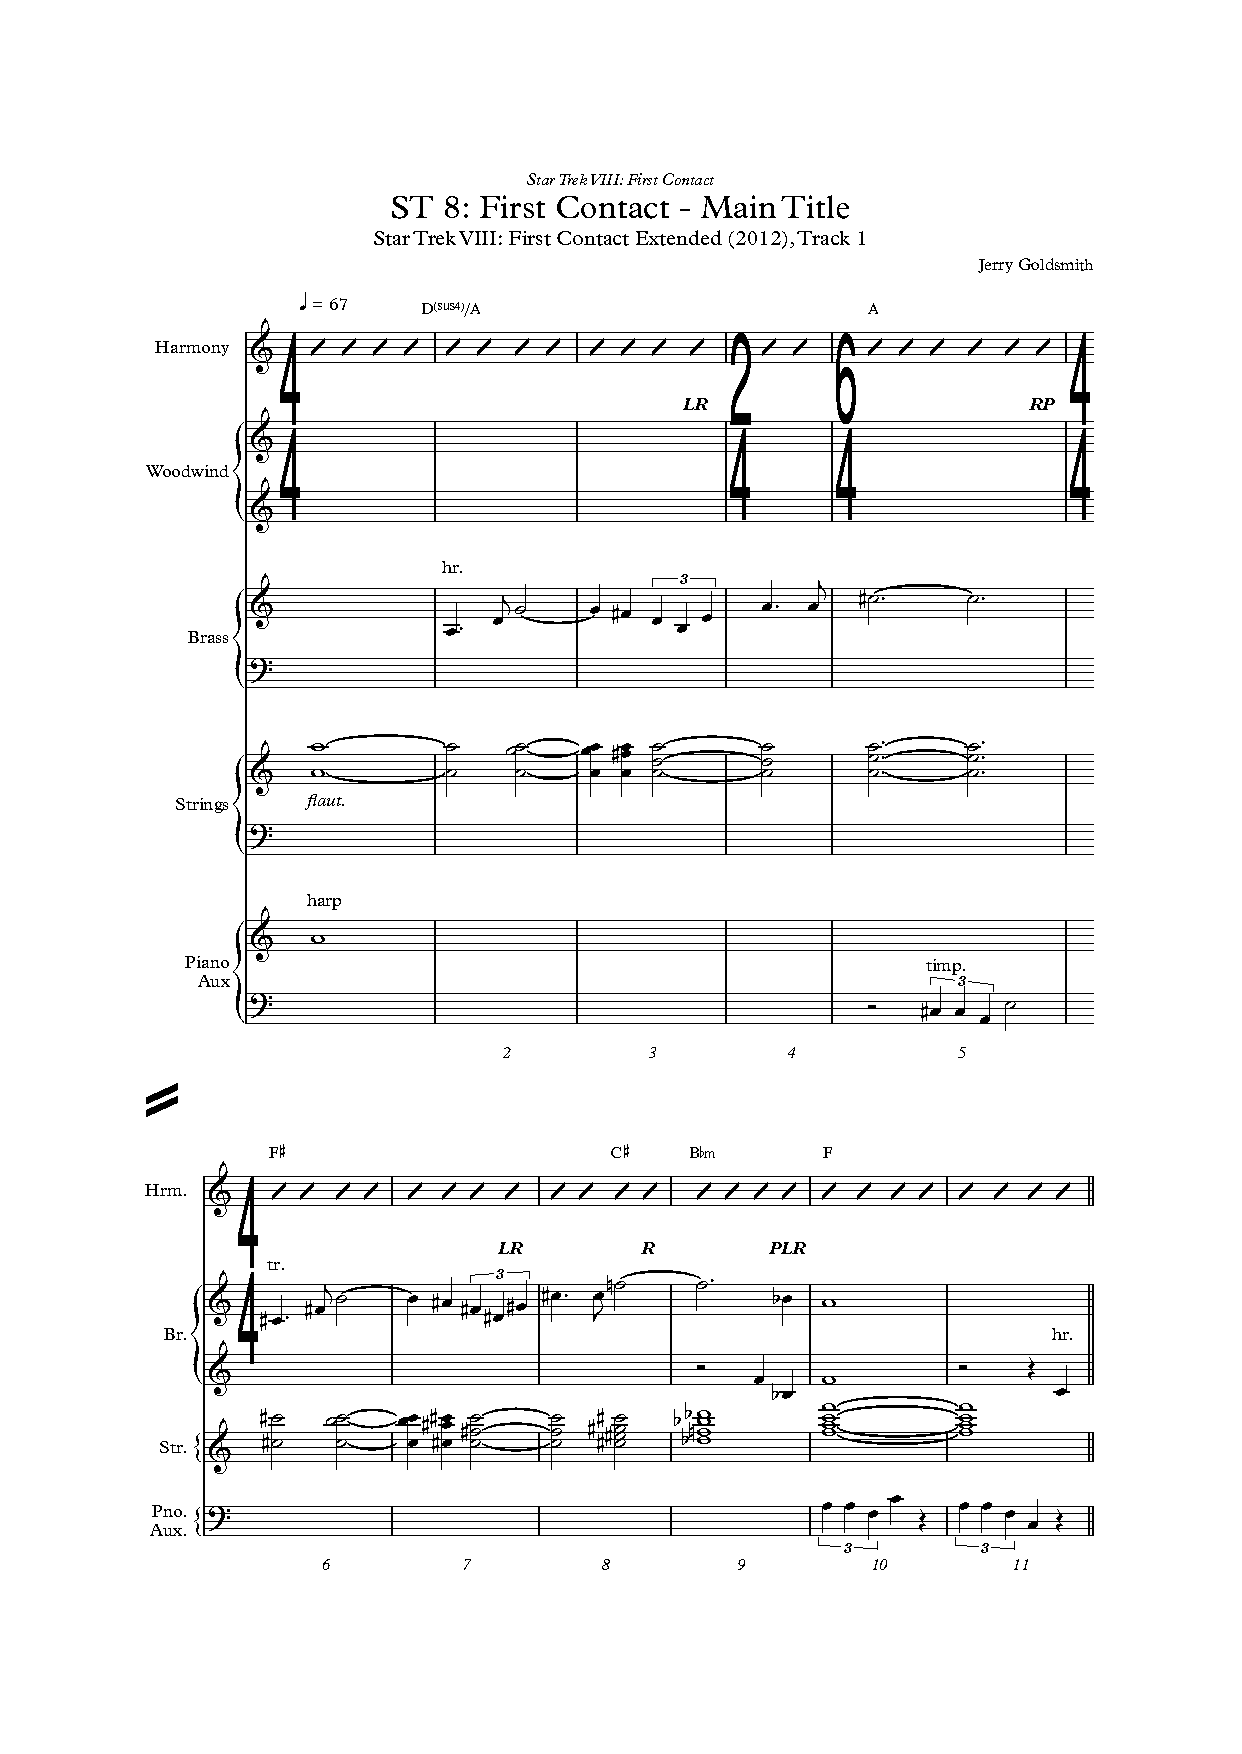
\includepdf[pages=-,pagecommand=\thispagestyle{fancy}]{pdf/ST8/ST08_First_Contact_Main_Title.pdf}

% Reviewed